\documentclass[11pt,a4paper]{article}\usepackage[]{graphicx}\usepackage[]{color}
% maxwidth is the original width if it is less than linewidth
% otherwise use linewidth (to make sure the graphics do not exceed the margin)
\makeatletter
\def\maxwidth{ %
  \ifdim\Gin@nat@width>\linewidth
    \linewidth
  \else
    \Gin@nat@width
  \fi
}
\makeatother

\definecolor{fgcolor}{rgb}{0.345, 0.345, 0.345}
\newcommand{\hlnum}[1]{\textcolor[rgb]{0.686,0.059,0.569}{#1}}%
\newcommand{\hlstr}[1]{\textcolor[rgb]{0.192,0.494,0.8}{#1}}%
\newcommand{\hlcom}[1]{\textcolor[rgb]{0.678,0.584,0.686}{\textit{#1}}}%
\newcommand{\hlopt}[1]{\textcolor[rgb]{0,0,0}{#1}}%
\newcommand{\hlstd}[1]{\textcolor[rgb]{0.345,0.345,0.345}{#1}}%
\newcommand{\hlkwa}[1]{\textcolor[rgb]{0.161,0.373,0.58}{\textbf{#1}}}%
\newcommand{\hlkwb}[1]{\textcolor[rgb]{0.69,0.353,0.396}{#1}}%
\newcommand{\hlkwc}[1]{\textcolor[rgb]{0.333,0.667,0.333}{#1}}%
\newcommand{\hlkwd}[1]{\textcolor[rgb]{0.737,0.353,0.396}{\textbf{#1}}}%
\let\hlipl\hlkwb

\usepackage{framed}
\makeatletter
\newenvironment{kframe}{%
 \def\at@end@of@kframe{}%
 \ifinner\ifhmode%
  \def\at@end@of@kframe{\end{minipage}}%
  \begin{minipage}{\columnwidth}%
 \fi\fi%
 \def\FrameCommand##1{\hskip\@totalleftmargin \hskip-\fboxsep
 \colorbox{shadecolor}{##1}\hskip-\fboxsep
     % There is no \\@totalrightmargin, so:
     \hskip-\linewidth \hskip-\@totalleftmargin \hskip\columnwidth}%
 \MakeFramed {\advance\hsize-\width
   \@totalleftmargin\z@ \linewidth\hsize
   \@setminipage}}%
 {\par\unskip\endMakeFramed%
 \at@end@of@kframe}
\makeatother

\definecolor{shadecolor}{rgb}{.97, .97, .97}
\definecolor{messagecolor}{rgb}{0, 0, 0}
\definecolor{warningcolor}{rgb}{1, 0, 1}
\definecolor{errorcolor}{rgb}{1, 0, 0}
\newenvironment{knitrout}{}{} % an empty environment to be redefined in TeX

\usepackage{alltt}
\usepackage[top=1.00in, bottom=1.0in, left=1.1in, right=1.1in]{geometry}
\usepackage{graphicx}
\usepackage[numbers]{natbib}
\bibliographystyle{..//..//references/styles/nature.bst}

\usepackage[export]{adjustbox}
\IfFileExists{upquote.sty}{\usepackage{upquote}}{}
\begin{document}


\includegraphics[width=0.5\textwidth, right]{AA_logo.jpg}
\noindent 1300 Centre Street\\
\noindent Boston, MA, 20131\\

\vspace{1.5ex}

\pagenumbering{gobble}

\noindent{Dear Dr. Gibson:}
\vspace{3ex}\\
\noindent Please consider our manuscript, `False spring damage to temperate tree saplings is amplified with winter warming', as a Research Article for the \textit{Journal of Ecology}. \\

\noindent Biological spring is advancing with climate change but late spring freeze dates are not predicted to advance at the same rate, leading to renewed interest in late spring freeze events---commonly called `false springs'---which shape the life history of many temperate and boreal plant species. Additionally, over-winter chilling is predicted to decrease with warming winters, which could impact plant phenology and, ultimately, growth. \\

\noindent Here, we present an experiment on the interplay of false springs and warmer winters (generally expected to reduce chilling) across eight temperate deciduous tree species examining a suite of phenological, growth and leaf tissue traits. We found that false springs slowed budburst to leafout timing---extending the period of maximum freezing risk, increased damage to the shoot apical meristem, and decreased leaf toughness, leaf thickness and chlorophyll content. Chilling accelerated budburst and leafout, even under false spring conditions, thus chilling compensated for the adverse phenological effects of false springs. Despite major shifts in phenology from false springs and chilling we did not find evidence of phenological reordering within a community. Our results instead suggest climate change will reshape forest communities through impacts on growth and leaf traits from the coupled effects of false springs and decreased over-winter chilling under future climate change.\\

\noindent We believe our research is important and timely because our findings contribute to fundamental knowledge on how chilling and freeze events shape tree growth across species, and suggest climate change could diminish or reverse the positive effects of carbon storage in temperate forests. Damage from false spring events in conjunction with decreases in over-winter chilling may have cascading effects to pollinators, nutrient cycling and carbon uptake as well as forest recruitment. \\ 

\noindent This manuscript is not under consideration elsewhere. Both authors approved of this version for submission. We hope that you will find it suitable for publication in the \textit{Journal of Ecology}. Thank you for your consideration. \\

\vspace{1.5ex}
\noindent Sincerely, \\
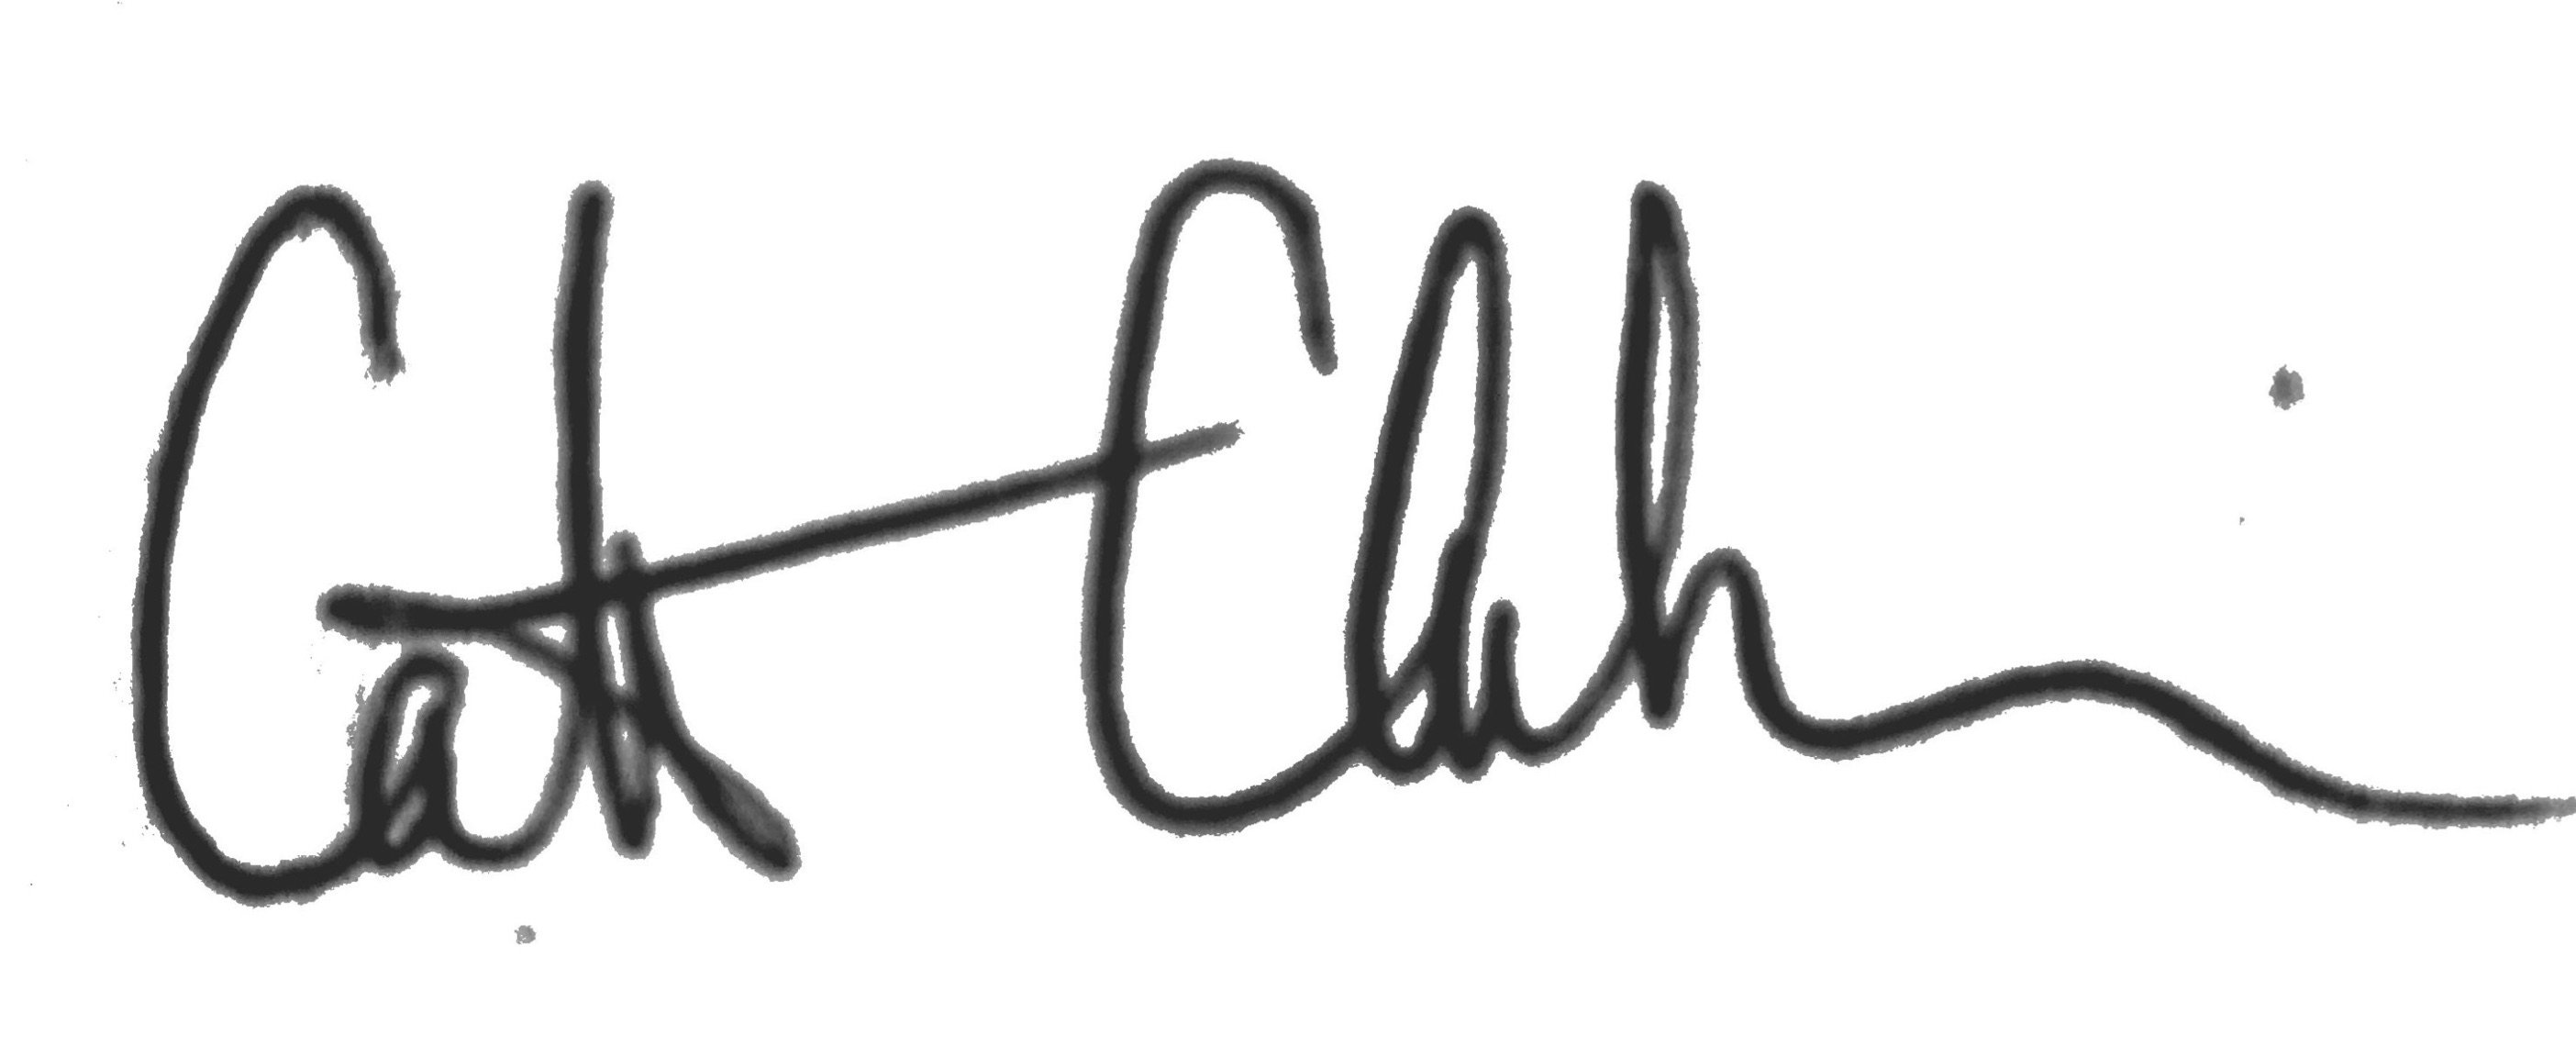
\includegraphics[width=0.2\textwidth]{full_signature.jpg} \\
\noindent Catherine Chamberlain (on behalf of my co-authors)
\vspace{2ex}\\
\noindent Authors:\\
C. J. Chamberlain $^{1,2}$ \& E. M. Wolkovich $^{1,2,3}$
\vspace{2ex}\\
\emph{Author affiliations:}\\
$^{1}$Arnold Arboretum of Harvard University, 1300 Centre Street, Boston, Massachusetts, USA; \\
$^{2}$Organismic \& Evolutionary Biology, Harvard University, 26 Oxford Street, Cambridge, Massachusetts, USA; \\
$^{3}$Forest \& Conservation Sciences, Faculty of Forestry, University of British Columbia, 2424 Main Mall, Vancouver, BC V6T 1Z4\\
\vspace{2ex}
$^*$Corresponding author: 248.953.0189; cchamberlain@g.harvard.edu\\

\bibliography{..//..//references/chillfreeze.bib}

\end{document}
